%%falta:
% corchetes formula
\section{Caracterización de componentes pasivos}

\subsection{Inductancia}
A continuación, se realizará un estudio acerca del comportamiento de una bobina, observando como varían sus magnitudes según la frecuencia y analizando sus circuitos equivalentes.\par En un sistema simplificado, la bobina sólo tiene un componente inductivo, sin embargo, dicho planteo dista en gran medida de la realidad donde, debido en gran medida a su fabricación, las inductancias tendrán tanto componentes resistivos como capacitivos. \par Las características previamente mencionadas nos llevarán a plantear distintos circuitos equivalentes. Se analizará cual de ellos refleja en mejor medida la práctica experimental realizada.

Para comenzar, se realiza el estudio de las magnitudes propias del inductor en función de la frecuencia. \par Las frecuencias utilizadas fueron detectadas ya que eran las que permitían ver con claridad como variaba la fase. Las mediciones se tomaron en el modo serie del analizador de impedancias, las mismas se pueden apreciar en la tabla (\ref{table:Rta_en_frecuencia_inductor}).

La inductancia provista por la cátedra tiene un valor nominal de $500\mu H$.
\par
Se plantea el siguiente circuito equivalente:

%circuito equivalente Inductancia
\begin{figure}[H]
\centering
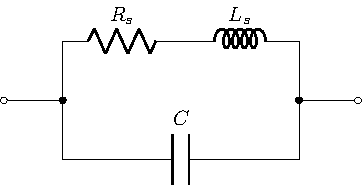
\includegraphics[width=6cm,height=4cm]{Ejercicio_1(Germo)/Circuitos/circuito_equivalente_inductancia.pdf}
\label{fig:circuito_equivalente_inductancia}
\caption{Circuito equivalente planteado para un inductor}
\end{figure}
%~circuito equivalente Inductancia

Al ser las bobinas un conjunto de espiras enrolladas una gran cantidad de vueltas, el componente resistivo de la inductancia se debe a la resistencia eléctrica del material utilizado en su fabricación. También, se podría considerar la resistencia propia de los terminales.
Por otro lado, debido a que constructivamente cada una de las vueltas de la bobina están aisladas eléctricamente entre si debido al barniz que recubre el material y a la pequeña diferencia de tensión, se puede apreciar el comportamiento de un capacitor entre vuelta y vuelta del cable.
%% Tabla inductor
 \begin{center}
     \begin{table}[H]
     \centering
     \renewcommand{\arraystretch}{1.1}
     \scalebox{0.7}{
         \begin{tabular}{ c c c c c c }
            \hline 
             $\bm{f_S[Hz]}$ &  $\bm{L_S[mH]}$ & $\bm{Q}$& $\bm{R_S[\Omega]}$ & $\bm{|Z|[\Omega]}$ & $\bm{\theta}[^\circ]$ \\
             \hline
                10		& 0.490        & 0.0    & 0.91 		& 0.96  & 18.7   \\
				100 	& 0.480       & 3.0   	 & 0.10  	& 0.32  & 72.0     \\
				1K    & 0.480         & 16.6	& 0.18 		& 3.02  & 86.0     \\
				5K    & 0.485        & 25.8 	& 0.59		 & 15.23 & 87.8   \\
				10K   & 0.482        & 26.0     & 1.16 		& 30.32 & 87.8   \\
				20K   & 0.478       & 23.8 		& 2.52 		& 60.11 & 87.6   \\
				30K   & 0.474       & 22.1 		& 4.04 		& 89.35 & 87.4  \\
				50K   & 0.467        & 19.5		 & 7.50 		 & 146.70 & 87.1  \\
				75K   & 0.462       & 16.7 		& 13.00   	& 217.80 & 86.6  \\
				100K  & 0.459       & 14.4 		& 20.00  	 & 289.20 & 86.0   \\
				200K  & 0.466       & 8.6  		& 67.70 	& 589.50 & 83.4    \\
				400K  & 0.529        & 4.1 		 & 322 		 & 1368  & 76.4   \\
				450K  & 0.556        & 3.5 		 & 450  	& 1635  & 74.1   \\
				500K  & 0.589        & 2.9 		 & 632 		 & 1954  & 71.2  \\
				550K  & 0.627        & 2.4  	& 893  		& 2344  & 67.6    \\
				600K  & 0.669        & 2.0    & 1281 		& 2829  & 63.1   \\
				650K  & 0.708        & 1.5 		 & 1868 	& 3442  & 57.1    \\
				700K  & 0.724       & 1.2  		& 2763 		& 4217  & 49.1    \\
				725K  & 0.711        & 1.0  	  & 3356	 & 4664  & 44.0    \\
				750K  & 0.671       & 0.8 		 & 4060 	& 5147  & 38.0    \\
				775K  & 0.595       & 0.6 		 & 4831 	& 5633  & 31.0       \\
				800K  & 0.472       & 0.4 		 & 5608 	& 6089  & 22.9       \\
				825K  & 0.301       & 0.2  		& 6264 		& 6456  & 14.0       \\
				850K  & 0.094        & 0.1  	& 6653		& 6672  & 4.4        \\
				855K  & 0.053       & 0.0  		  & 6692	 & 6698  & 2.5        \\
				862K5 & -0.100         & 0.0    & 6715 		& 6715  & -0.5       \\
				870K  & -0.719       & 0.1 		 & 6706 	& 6718  & -3.4        \\
				875K  & -0.111      & 0.1  		& 6677 		& 6705  & -5.3       \\
				900K  & -0.290      & 0.3  		& 6356 		& 6563  & -14.4      \\
				925K  & -0.421      & 0.4 		 & 5787		 & 6282  & -22.9      \\
				950K  & -0.500         & 0.6  	& 5114 		& 5921  & -30.3       \\
				1M    & -0.549      & 0.9  		& 3820		 & 5146  & -42.1      \\
				1M1  & -0.470      & 1.5  		& 2132		 & 3884  & -56.7      \\
				1M2  & -0.368      & 2.1  		& 1306 		& 3068  & -64.8      \\
				1M3   & -0.291      & 2.7  		& 874  		& 2531  & -69.8      \\
				1M4  & -0.235      & 3.3 		 & 626  	& 2159  & -73.2     \\
				2M    & -0.093      & 6.7 		 & 175 		 & 1179  & -81.5       \\
				4M    & -19.79$*10^-3$  & 16.8 		& 29.6		 & 498.4 & -86.6     \\
				10M   & -2.893$*10^-3$ & 27.3 		& 6.7  		& 181.9 & -87.9     \\
            \hline 
        \end{tabular}
        }
        \caption{Magnitudes del inductor en función de la frecuencia}
        \label{table:Rta_en_frecuencia_inductor}
    \end{table}
\end{center}
%%~Tabla inductor
A continuación, para calcular empíricamente el módulo de la impedancia se considerará la disposición planteada en el circuito equivalente, donde se encuentra el capacitor en paralelo con la resistencia y la inductancia, obteniéndose: 
\begin{equation}
|Z|= \frac{R_S+\$L}{\$^2LC+\$R_SC+1}
\end{equation}
Mientras que la fase se obtendrá mediante la siguiente ecuación:
\begin{equation}
\theta= arctg(\frac{Im(Z)}{Re(Z)})
\end{equation}
Para nuestro modelo se tomaron tres valores distintos posibles de capacitancia, dichos valores fueron seleccionadas ya que eran los que hacían que la impedancia se asemejara más a la obtenida empíricamente. Los valores utilizados fueron $1nF$, $1pF$ y $1fF$.

La relación entre las impedancias obtenidas tomando dichos valores y la empírica se grafica a continuación.

%grafico relacion Zs
\begin{figure}[H]
\centering
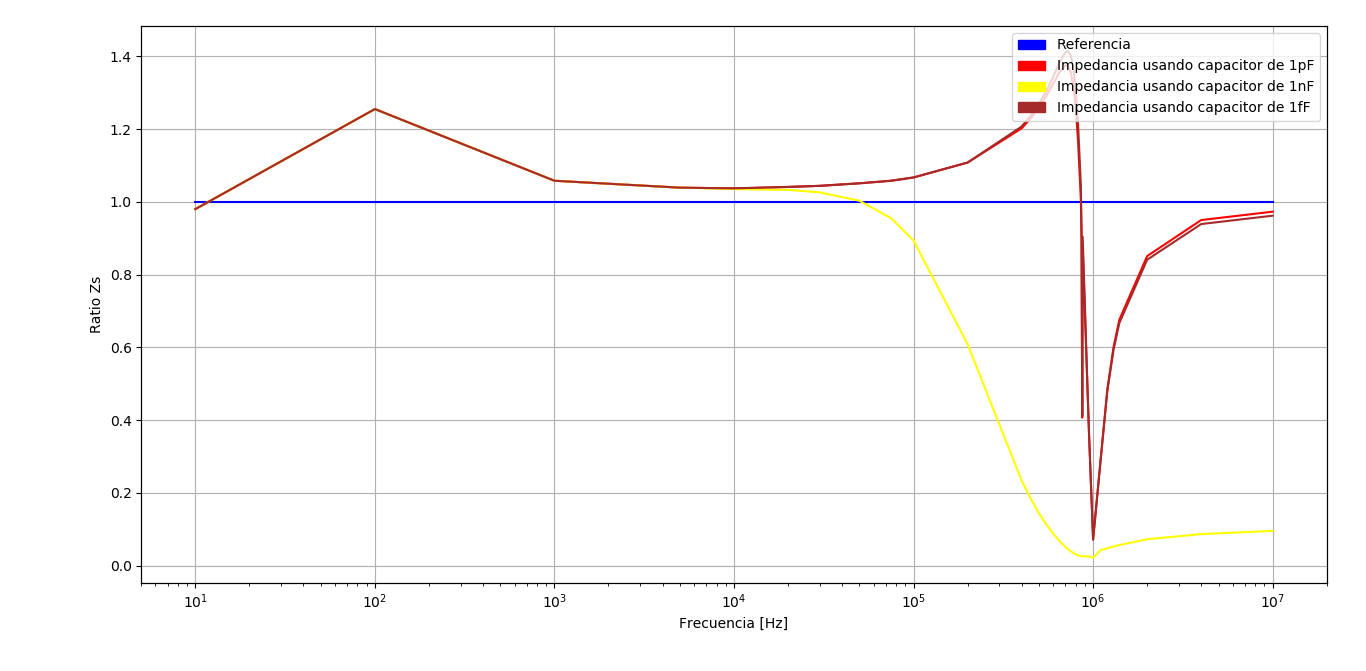
\includegraphics[width=1\textwidth]{Ejercicio_1(Germo)/Grafico/relacionZs.png}
\label{fig:relacionZs}
\caption{Ratio entre las impedancias para distintos valores de C}
\end{figure}
%~grafico relacion Zs


Consiguientemente, se decidió tomar una capacitor de capacidad $1pF$ ya que era el que producía una impedancia de mayor relación con la obtenida mediante el analizador de impedancia. Se grafica la impedancia y fase obtenida empíricamente con la obtenida a través de los cálculos provistos arriba considerando el capacitor anteriormente mencionado.

%grafico |Z| y fase
\begin{figure}[H]
\centering
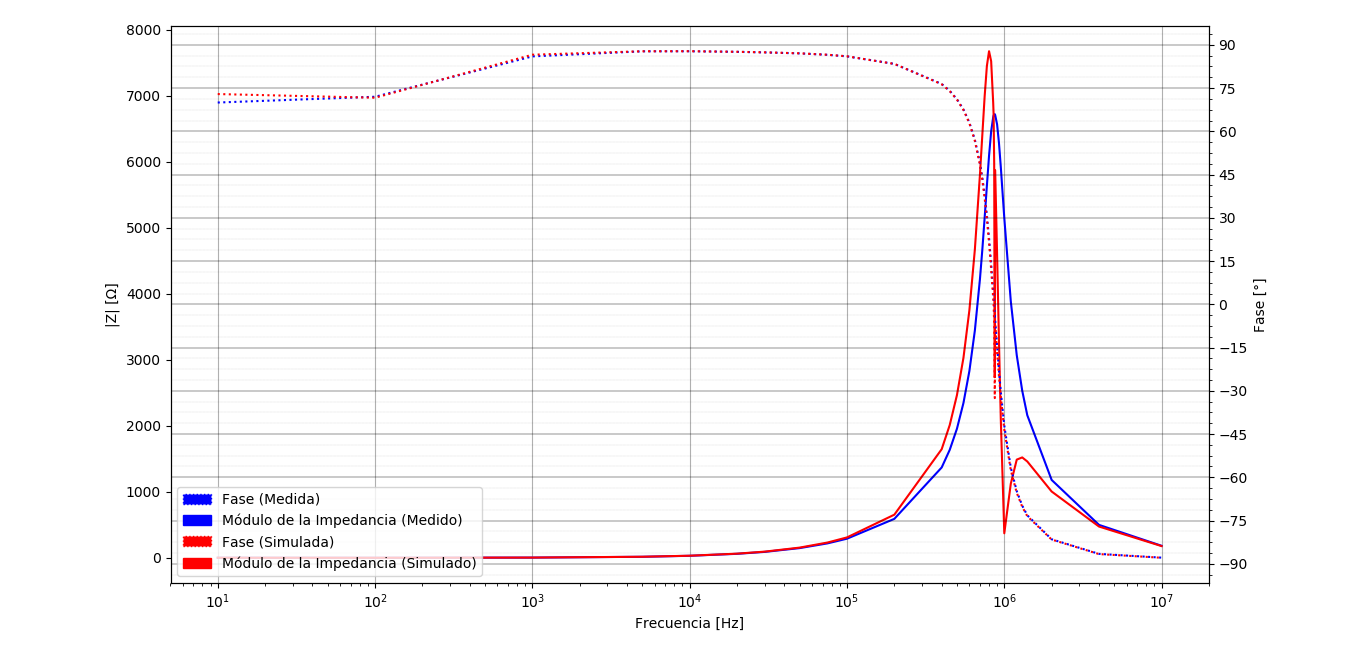
\includegraphics[width=1\textwidth]{Ejercicio_1(Germo)/Grafico/Inductancia_relacion_entre_Z_y_fases.png}
\label{fig:Inductancia_relacion_entre_Z_y_fases}
\caption{Módulo y fase de Z (Simulado vs Empírico)}
\end{figure}
%~grafico |Z| y fase

Debido a que no es posible ver con claridad las variaciones si se toma solamente el módulo de la impedancia, se analiza a continuación como varía la resistencia serie presente en el circuito. Se compara la obtenida mediante el analizador de impedancia en contraste con la parte real del módulo, que representaría la variación de dicho componente ya que es el único de valor 'real'.\par
Por otro lado, en el mismo gráfico se muestra el valor de la inductancia serie para no sobrecargar el informe de figuras.

%grafico |Z| y fase
\begin{figure}[H]
\centering
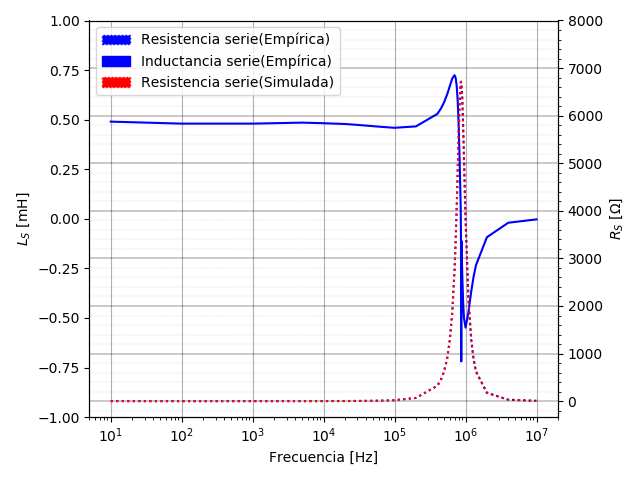
\includegraphics[width=0.75\textwidth]{Ejercicio_1(Germo)/Grafico/Inductancia_relacion_entre_L_s_y_R_s.png}
\label{fig:Inductancia_relacion_entre_L_s_y_R_s}
\caption{Variación $R_S$ (Simulado vs Empírico) / $L_S$ }
\end{figure}
%~grafico |Z| y fase

Como conclusión del análisis gráfico, se grafica el factor de calidad de la inductancia obtenida empíricamente en contraposición con su par obtenido de manera teórica mediante la fórmula que se presenta continuación.

\begin{equation}
Q= \frac{\$L}{R}
\end{equation}

%grafico |Z| y fase
\begin{figure}[H]
\centering
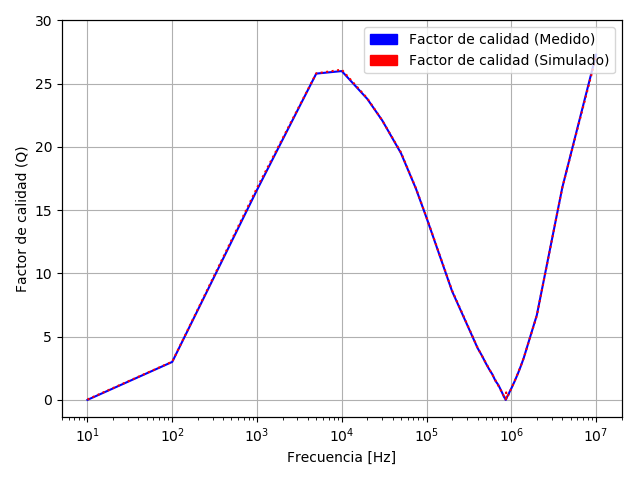
\includegraphics[width=0.75\textwidth]{Ejercicio_1(Germo)/Grafico/QteovsQcalc.png}
\caption{Factor de calidad del inductor}
\label{fig:QteovsQcalc}
\end{figure}
%~grafico |Z| y fase

\subsubsection*{Conclusiones}


\subsection{Capacitor}
Se procederá a realizar el mismo análisis planteado anteriormente para una inductancia pero, para este caso con un capacitor, analizando como varían sus magnitudes según la frecuencia a la que trabaja y el estudio de sus circuitos equivalentes.

Para comenzar, se realiza el estudio de las magnitudes propias del capacitor en función de la frecuencia. \par Las frecuencias utilizadas fueron detectadas ya que eran las que permitían ver con claridad como variaba la fase. Las mediciones se tomaron en el modo paralelo del analizador de impedancias por lo que se medirán conductancias. Las mismas se pueden apreciar en la tabla (\ref{table:Rta_en_frecuencia_capacitor}).

El capacitor utilizado fue el provisto por la cátedra para el Trabajo Práctico N°1 de $2.2nF$.
\par
Se plantea el siguiente circuito equivalente:

%circuito equivalente capacitor
\begin{figure}[H]
\centering
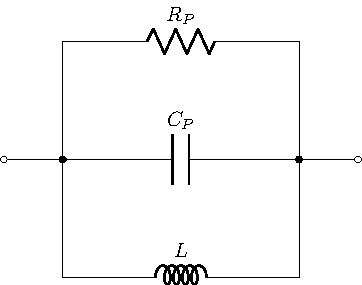
\includegraphics[width=6cm,height=4cm]{Ejercicio_1(Germo)/Circuitos/circuito_equivalente_capacitor_todoparalelo.pdf}
\label{fig:circuito_equivalente_capacitor_todoparalelo}
\caption{Circuito equivalente planteado para un capacitor}
\end{figure}
%~circuito equivalente capacitor
La resistencia observada se debe a la resistencia eléctrica del material del componente(film) .También, se podría considerar la resistencia propia de los terminales. \par

%% Tabla capacitor
 \begin{center}
 
     \begin{table}[H]
     \centering
     \renewcommand{\arraystretch}{1.1}
     \scalebox{0.7}{
         \begin{tabular}{ c c c c c c c c }
            \hline 
             $\bm{f_P[Hz]}$ &  $\bm{C_P[nF]}$ & $\bm{D}$& $\bm{R_P[S]}$ & $\bm{|Z|[S]}$ & $\bm{\theta}[^\circ]$ \\

             \hline
             10   & 2.20  & 0.000 & 0.00       & 0.14$\mu$   & 89.9  \\
			100  & 2.27 & 0.010 & 0.00       & 1.43$\mu$   & 89.90 \\
			1K   & 2.26 & 0.004 & 0.05$\mu$   & 14.22$\mu$  & 89.80 \\
			5K   & 2.25 & 0.007 & 0.49$\mu$   & 70.73$\mu$  & 89.60 \\
			10K  & 2.24 & 0.007 & 1$\mu$ & 0.14$m$ & 89.56 \\
			20K  & 2.23 & 0.010 & 3$\mu$ & 0.28$m$ & 89.42 \\
			30K  & 2.23 & 0.011 & 5$\mu$  & 0.42$m$    & 89.35 \\
			50K  & 2.22 & 0.013 & 9$\mu$  & 0.70$m$  & 89.28 \\
			75K  & 2.21 & 0.014 & 14$\mu$  & 1.04$m$   & 89.22 \\
			100K & 2.21 & 0.014 & 19$\mu$   & 1.38$m$   & 89.21 \\
			200K & 2.19 & 0.015 & 42$\mu$   & 2.75$m$  & 89.30 \\
			400K & 2.18 & 0.016 & 88$\mu$   & 5.47$m$   & 89.08 \\
			450K & 2.17 & 0.016 & 100$\mu$    & 6.15$m$  & 89.07 \\
			500K & 2.17 & 0.016 & 111$\mu$   & 6.82$m$  & 89.06 \\
			550K & 2.12 & 0.017 & 124$\mu$   & 7.40$m$    & 89.06 \\
			650K & 2.17 & 0.017 & 149$\mu$   & 8.84$m$   & 89.04 \\
			750K & 2.16 & 0.017 & 173$\mu$   & 10.20$m$   & 89.03 \\
			800K & 2.16 & 0.017 & 186$\mu$   & 10.87$m$  & 89.02 \\
			900K & 2.16 & 0.017 & 210$\mu$    & 12.22$m$  & 89.01 \\
			1M   & 2.16 & 0.018 & 240$\mu$    & 13.57$m$  & 89.00 \\
			1M2  & 2.16 & 0.018 & 290$\mu$    & 16.27$m$  & 88.97 \\
			2M   & 2.16 & 0.019 & 520$\mu$    & 27.12$m$ & 88.90 \\
			4M   & 2.2  & 0.023 & 1.270$m$   & 55.38$m$  & 88.68 \\
			7M   & 2.3  & 0.032 & 3.200$m$    & 101.05$m$ & 88.16 \\
			9M   & 2.43 & 0.039 & 0.005   & 0.13  & 87.70 \\
			11M  & 2.63 & 0.050 & 0.009   & 0.18   & 87.10 \\
			12M  & 2.76 & 0.057 & 0.012   & 0.21   & 86.70 \\
			13M  & 2.91 & 0.065 & 0.015   & 0.24   & 86.30 \\
            \hline 
        \end{tabular}
        }
        \caption{Magnitudes del capacitor en función de la frecuencia}
        \label{table:Rta_en_frecuencia_capacitor}
    \end{table}
\end{center}
%%~Tabla capacitor
A continuación, para calcular empíricamente el módulo de la impedancia se considerará la disposición planteada en el circuito equivalente, donde se encuentra en paralelo el capacitor, la resistencia y la inductancia, obteniéndose: 

\begin{equation}
|Z|= \frac{(1+R_P\$C)L\$}{\$^2LC+\$R_PC+1}
\end{equation}

Mientras que la fase se obtendrá mediante la siguiente ecuación:

\begin{equation}
\theta= arctg(\frac{Im(Z)}{Re(Z)})
\end{equation}

Para nuestro modelo se tomaron dos valores distintos posibles de inductancia, dichos valores fueron seleccionadas ya que eran los que hacían que la impedancia se asemejara más a la obtenida empíricamente. Los valores utilizados fueron $1nH$ y $2.25nH$.

La relación entre las impedancias obtenidas tomando dichos valores y la empírica se grafica a continuación.

%grafico |Z| y fase
\begin{figure}[H]
\centering
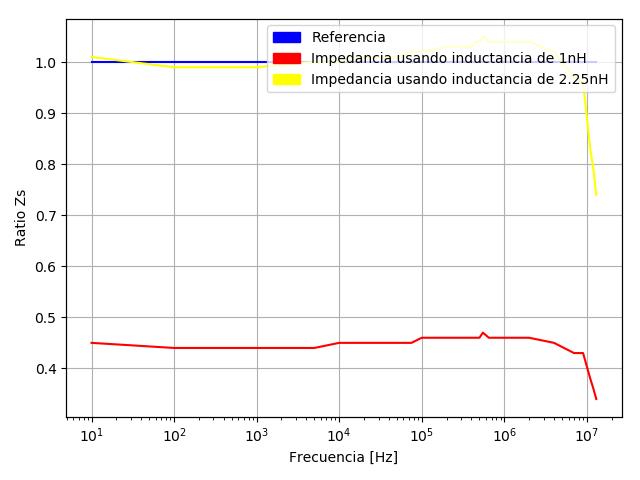
\includegraphics[width=1\textwidth]{Ejercicio_1(Germo)/Grafico/capacitor_relacion_entre_Z.png}
\label{fig:capacitor_relacion_entre_Z}
\caption{Ratio entre las impedancias para distintos valores de L}
\end{figure}
%~grafico |Z| y fase


Consiguientemente, se decidió tomar una inductancia de valor $2.25nH$ ya que era el que producía una impedancia de mayor relación con la obtenida mediante el analizador de impedancia. Se grafica la impedancia y fase obtenida empíricamente con la obtenida a través de los cálculos provistos arriba considerando el capacitor anteriormente mencionado.

%grafico |Z| y fase
\begin{figure}[H]
\centering
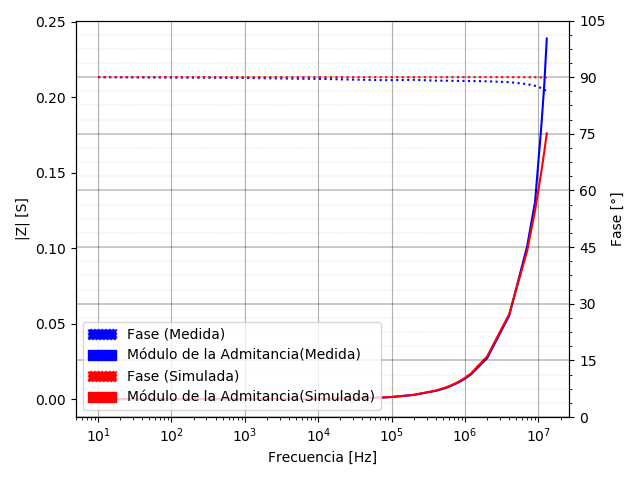
\includegraphics[width=0.75\textwidth]{Ejercicio_1(Germo)/Grafico/Capacitor_relacion_entre_Z_y_fases.png}
\label{fig:Capacitor_relacion_entre_Z_y_fases}
\caption{Módulo y fase de Z (Simulado vs Empírico)}
\end{figure}
%~grafico |Z| y fase

Debido a que no es posible ver con claridad las variaciones si se toma solamente el módulo de la impedancia, se analiza a continuación como varía la resistencia paralela presente en el circuito. Se compara la obtenida mediante el analizador de impedancia en contraste con la parte real del módulo, que representaría la variación de dicho componente ya que es el único de valor 'real'.\par
Por otro lado, en el mismo gráfico se muestra el valor de la capacitancia paralela para no sobrecargar el informe de figuras.
%grafico |Z| y fase
\begin{figure}[H]
\centering
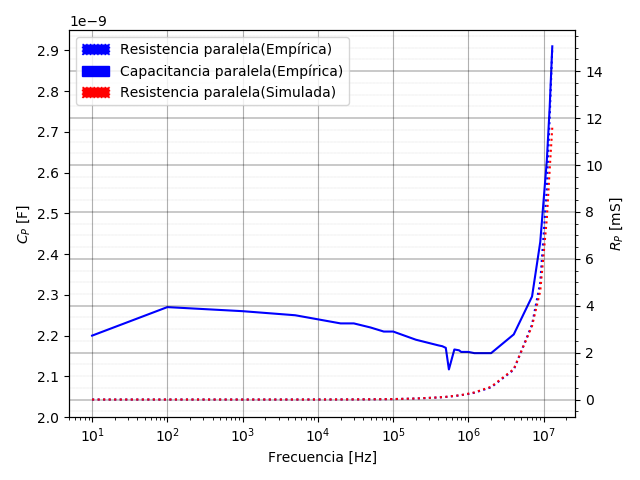
\includegraphics[width=0.75\textwidth]{Ejercicio_1(Germo)/Grafico/capacitor_relacion_C_P_y_R_p.png}
\label{fig:capacitor_relacion_C_P_y_R_p}
\caption{Variación $R_P$ (Simulado vs Empírico) / $C_P$ }
\end{figure}
%~grafico |Z| y fase

Como conclusión del análisis gráfico, se grafica el factor de pérdidas del capacitor obtenido empíricamente en contraposición con su par obtenido de manera teórica mediante la fórmula que se presenta continuación.

\begin{equation}
Q= \frac{\$C}{R_P}
\end{equation}
\begin{equation}
D= \frac{1}{Q}
\end{equation}

%grafico |Z| y fase
\begin{figure}[H]
\centering
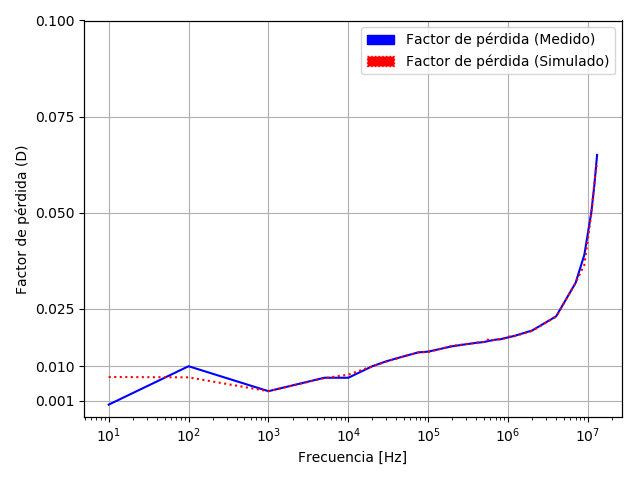
\includegraphics[width=0.75\textwidth]{Ejercicio_1(Germo)/Grafico/capacitor_factor_de_perdida.png}
\label{fig:capacitor_factor_de_perdida}
\caption{Factor de pérdidas del capacitor}
\end{figure}
%~grafico |Z| y fase

\subsubsection*{Conclusiones}

